\documentclass[12pt,Bold,letterpaper,TexShade]{mcgilletdclass}
\usepackage[utf8]{inputenc}
\usepackage{amsmath}
\usepackage{amsfonts}
\usepackage{amssymb}
\usepackage{graphicx}
\usepackage{braket}
\usepackage{natbib}
\usepackage{bm}
\usepackage[toc,page]{appendix}
\pagenumbering{arabic}
\linespread{1.3}



\SetTitle{\huge{Simulating Optical Pumping\\in the Laser Spectroscopy \\Experiment at TRIUMF}}%
\SetAuthor{Julien Refour}%
\SetDegreeType{Masters of Science}%
\SetDepartment{Department of Physics}%
\SetUniversity{McGill University}%
\SetUniversityAddr{Montreal,Quebec}%
\SetThesisDate{2017-09-15}%
\SetRequirements{Requirements Statement}%
\SetCopyright{Copyright Statement}%



%% Input any special commands below
%\newcommand{\Kron}[1]{\ensuremath{\delta_{K}\left(#1\right)}}
\listfiles%
\begin{document}

\maketitle%

\begin{romanPagenumber}{2}%

\SetDedicationName{\MakeUppercase{Dedication}}%
\SetDedicationText{This document is dedicated to the graduate students of the McGill University.}%
\Dedication%

\SetAcknowledgeName{\MakeUppercase{Acknowledgements}}%
\SetAcknowledgeText{Acknowledgments, if included, must be written in complete sentences.  Do not use direct address.  For example, instead of Thanks, Mom and Dad!, you should say I thank my parents. }%
\Acknowledge%


%%%%%%%%%%%%%%%%%%%%%%%%%%%%%%%%%%%%%%%%%%%%%%%%%%%%%
%%         English Abstract                        %%
%%%%%%%%%%%%%%%%%%%%%%%%%%%%%%%%%%%%%%%%%%%%%%%%%%%%%
\SetAbstractEnName{\MakeUppercase{Abstract}}%
\SetAbstractEnText{ Abstract in English and French are required. The text of the abstract in English begins here.}
\AbstractEn%

%%%%%%%%%%%%%%%%%%%%%%%%%%%%%%%%%%%%%%%%%%%%%%%%%%%%%
%%         French Abstract                         %%
%%%%%%%%%%%%%%%%%%%%%%%%%%%%%%%%%%%%%%%%%%%%%%%%%%%%%
\SetAbstractFrName{\MakeUppercase{ABR\'{E}G\'{E}}}%
\SetAbstractFrText{ The text of the abstract in French begins here.  }%
\AbstractFr%

\TOCHeading{\MakeUppercase{Table of Contents}}%
\LOTHeading{\MakeUppercase{List of Tables}}%
\LOFHeading{\MakeUppercase{List of Figures}}%
\tableofcontents %
\listoftables %
\listoffigures %

\end{romanPagenumber}

%\mainmatter %
 
\chapter{Introduction}


	



\chapter{Theory of Laser Spectroscopy}

\chapter{Theory of Laser Spectroscopy}
In this chapter, the theoretical background necessary to the understanding and simulation of a hyperfine spectrum is presented. In $\S$ \ref{AHF}, the features of a hyperfine spectrum are liked to physical properties a nucleus. Next, $\S$ \ref{ALI} outlines the way in which lasers interact with atoms
Note: Throughout this section, a variable written in a bold typeface is vector valued, while its non-bold counterpart is its magnitude. 
\section{Anatomy of A Hyperfine Spectrum}
\label{AHF}
\begin{figure}[h]
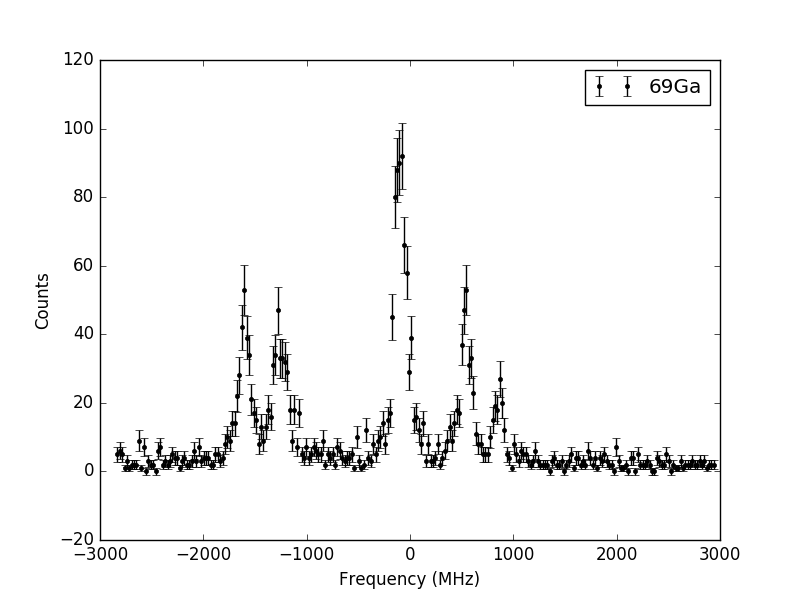
\includegraphics[width=\textwidth]{Graphics/ga69.png}
\caption{Hyperfine spectrum of Gallium-69 for the 4P$_{3/2}\rightarrow$5S$_{1/2}$ transition. Photon counts are shown on the vertical axis, while the horizontal axis gives relative frequency with respect to the fine transition. The errorbars are standard Poisson counting errors.}
\label{ga69}
\end{figure}
How can the properties of a hyperfine spectrum, such as that of $^{69}\mathrm{Ga}$ shown in Fig. \ref{ga69}, be translated into measurements of the physical properties of the nucleus? The hyperfine spectrum is, after all, the result of probing the electronic structure of the atom. The answer, of course, is that the electrons interact with the nucleus through several mechanisms, each of which will be described in this section. To begin, however, consider the following system: An electron transitions from a ground state $\ket{g}$ to an excited state $\ket{e}$. More precisely $\ket{g}$ and $\ket{e}$ are defined as 
\begin{align}
\ket{g} =& \ket{n_g,\mathrm{L_g,L_{g,z}}}\\
\ket{e} =& \ket{n_e,\mathrm{L_e,L_{e,z}}}
\end{align}
where $n_{g,e}$ are principal quantum numbers, $\bf{L_{g,e}}$ the orbital angular momenta, and L$_{g,e}^z$ the projections of the orbital angular momentum on an axis of quantization $z$. Next, if nucleus of the atom in which this transition is occurring has angular momentum $\bf{I}$, then a quantity, $\bf{F}$, can be defined as 

\begin{equation}
\bf{F_{g,e}} = \bf{I} + \bf{L_{g,e}}
\end{equation}
$\bf{F}$ describes the total angular momentum state of the atom, so $\ket{g}$ and $\ket{e}$ can be rewritten as

\begin{align}
\ket{g} =& \ket{n_g,\mathrm{F_g, F_{g,z}}}\\
\ket{e} =& \ket{n_e,\mathrm{F_e, F_{e,z}}}
\end{align}
For a fixed $\bf{I}$, $\bf{F}$ can range from $(-\mathrm{L+I})$ to $(\mathrm{L+I})$.
\subsection{Peak Energies}
The energy of the electrons depends on the various electron-nucleus interactions present in the atom. If for the purposes of this work, only three interactions produce measurable changes in the energies of the electron levels. These are the isotope, magnetic dipole and electric quadrupole shifts. There are higher order interactions (magnetic octopole, electric hexadecapole), however their effects are far below the resolution of the experimental set-up employed at TRIUMF. For example, the three interactions listed above lead to energy shifts on the order of roughly $10^{-7}-10^{-4}$ eV \cite{ModAN}. Higher order interactions are typically far below the resolution of the experiment, and thus are not considered in this work. 

\subsubsection*{Isotope Shift}
The isotope shift is measured with respect to a reference isotope. As neutrons are added or removed from a nucleus, the charge distribution, as well as the mass, of the nucleus changes. This leads to three different effects on the energies of the electrons. 

The change in the mass of the nucleus leads to what is known as the Mass shift, $\Delta E_M$. The mass shift between two isotopes with mass numbers A and A' is given by
\begin{equation}
\Delta E_M = \frac{m_{\mathrm{A}}-m_{\mathrm{A'}}}{2 m_{\mathrm{A}} m_{\mathrm{A'}}} \left(\sum_i\mathrm{\textbf{p}}_i +2 \sum_{i>j}\mathrm{\textbf{p}}_i \cdot \mathrm{\textbf{p}}_j \right)
\end{equation}
where $m_{\mathrm{A}}$ and $m_{\mathrm{A'}}$ are the isotope masses, and the $\textbf{p}_i$ are the electron momenta. The first term is due to the nucleus recoiling with the electrons when a photon is absorbed, while the second term deals with the electron-electron interactions.  

The change in the charge distribution of the nucleus produces the Field shift. While the typical nucleus is far smaller the wavefunction of a typical orbital electron, the effect is still important. The energy of a nucleus in the charge density produced by the electrons at the origin, $E_F$, is given by

\begin{equation}
E_F = \frac{Ze^2}{6 \epsilon_0}|\psi(0)|^2 \left\langle r_{ch}^2\right\rangle
\end{equation}
where $\epsilon_0$ is the permitivity of free space, $Z$ is the proton number, $e$ is the fundamental charge and $ \left\langle r_{ch}^2\right\rangle$ is the mean-square charge radius of the nucleus, defined as
\begin{equation}
 \left\langle r_{ch}^2\right\rangle = \frac{\int_0^{\infty}\rho(\mathbf{r})r^2dV}{\int_0^{\infty}\rho(\mathbf{r})dV}
\end{equation}
The field shift between two isotopes is then given by
\begin{equation}
\Delta E_F =  \frac{Ze^2}{6 \epsilon_0}\Delta|\psi(0)|^2 \Delta\left\langle r_{ch}^2\right\rangle
\end{equation}

In total, then, the isotope shift $\Delta E_{\mathrm{A,A}'}$ is given by
\begin{equation}
 \Delta E_{\mathrm{A,A'}} = \Delta E_M + \Delta E_F
\end{equation}
\subsubsection*{Magnetic Dipole Shift}
A nucleus with a non-zero nuclear spin $\bf{I}$  will have a magnetic dipole moment, given by

\begin{equation}
\boldsymbol{\mu}_{\mathrm{\bf{I}}} = g_{\mathrm{I}}\mu_{\mathrm{N}}\mathrm{\bf{I}}
\end{equation}

where $g_{\mathrm{I}}$ is the g-factor and $\mu_{\mathrm{N}}$ is the nuclear magneton. (REFERENCE NEEDED) The interaction of $\mu_{\mathrm{I}}$ with the magnetic field produced by the electrons, $\mathrm{\bf{B_e}}$, creates a shift in the energy of the orbiting electrons. Provided the electrons occupy an angular momentum state $\mathrm{\bf{L}} \neq 0$, the hamiltonian for this interaction is given by

\begin{equation}
\mathcal{H} = -\boldsymbol{\mu}_{\mathrm{\bf{I}}} \cdot \mathrm{\bf{B_e}}
\end{equation}

This interaction leads to a shift, $\Delta E_{\mu_I}$, in the energy of the atomic states by

\begin{equation}
\Delta E_{\mu_I} = \frac{AK}{2}
\end{equation}

where $K = \mathrm{F(F+1) - I(I+1) - L(L+1)}$ and 

\begin{equation}
A = \frac{\mu_{\mathrm{I}}\mathrm{B_e}}{\mathrm{IL}}
\end{equation}

\subsubsection*{Electric Quadrupole Shift}
The electric quadrupole moment is used to describe the distribution of charge in a nucleus. For a nucleus composed of $n$ protons and $\mathbf{I}\geq1$, the electric quadrupole moment, Q, is given by

\begin{equation}
\mathrm{Q} = \sum_i^n (3z_i^2-r_i^2)
\end{equation}
where $r_i^2 = x_i^2+y_i^2+z_i^2$. If Q $ < 0$, then the nucleus is stretched in the $x-y$ plane. If Q $ > 0$, then the nucleus is stretched along the $z-$axis. It is important to note that these deformations a symmetric with respect to an axis of symmetry, the $z-$axis in this case. Q $=0$ indicates that the nucleus is spherical. 

In reality, direct measurement of Q is not feasible, as the nucleus is rotating. Instead, the spectroscopic quadrupole, Q$_s$, is measured. Q$_s$ is defined as the projection of Q onto the axis of quantization of the nucleus, and is given by
\begin{equation}
\mathrm{Q}_s = \frac{\mathrm{I}(2\mathrm{I}-1)}{(\mathrm{I}+1)(2\mathrm{I}+3)}\mathrm{Q}
\end{equation}
The use of $Q_s$ as a measure of $Q$ is valid under the assumption that the nuclear deformation is axially symmetric. Additionally, it is assumed that the axis of symmetry has a well defined direction with respect to \textbf{I}.

The hamiltonian for the interaction between the spectroscopic electric quadrupole moment and the electric field produced by the electrons at the nucleus, $E_N$, is given by

\begin{equation}
\mathcal{H} = - \frac{1}{6}e\mathrm{Q}_s\nabla{E_N}
\end{equation}
where
\begin{equation}
\nabla{E_N} = \frac{\partial^2V}{\partial x_i\partial x_j}, \{x_j,x_k\} \in \{x,y,z\} \otimes \{x,y,z\}
\end{equation}
$e$ is the fundamental charge and $V$ is the electric potential. Recalling that the nuclear deformation is symmetric about the axis of quantization, the shift in energy is then given by

\begin{equation}
\Delta E_{\mathrm{Q_s}} = \frac{B}{4}\left[\frac{\frac{3}{2}K(K+1)-2\mathrm{I}(\mathrm{I}+1)\mathrm{L}(\mathrm{L}+1)}{\mathrm{I}(2\mathrm{I}-1)\mathrm{L}(2\mathrm{L}-1)}\right]
\label{B-eq}
\end{equation}
where $B$ is a hyperfine coefficient and is given by
\begin{equation}
B = e\mathrm{Q_s}\left\langle\frac{\partial^2V}{\partial z^2} \right\rangle
\end{equation}
Eq. \ref{B-eq} has singularities at \textbf{I} = $\frac{1}{2}$ and \textbf{L}=$\frac{1}{2}$. This captures the fact that in either case there is no coupling between the nucleus and the electrons, as an orbital angular momentum state of $\frac{1}{2}$ is isotropically distributed in space .

\subsubsection*{The Hyperfine Equation}
The resonant energy of a transition between $\ket{g}=\ket{n_g,\mathrm{\textbf{F}_g=\textbf{I} + \textbf{L}_g}}$ and $\ket{e}=\ket{n_e,\mathrm{\textbf{F}_e=\textbf{I} + \textbf{L}_e}}$ is then given by
\begin{equation}
E_{hfs} = E_{fs} +  \Delta E_{\mathrm{A,A'}}+\Delta E_{\mu_I}\Bigr|_{\mathrm{F_g},I,L_g}^{\mathrm{F_e},I,L_e}+\Delta E_{\mathrm{Q_s}}\Bigr|_{\mathrm{F_g},I,L_g}^{\mathrm{F_e},I,L_e}
\end{equation}

When a hyperfine spectrum is fit, the fit parameters which govern the locations of the peaks are the hyperfine parameters $A$ and $B$ for both $\ket{e}$ and $\ket{g}$, as well as what is known as the centroid, $\nu_0$. The centroid combines the fine structure energy and the isotope shift into one quantity. It is important to note that while the values of hyperfine coefficients can be directly linked to the physical properties of the nucleus, only the change in the centroid with respect to a reference isotope can be used to measure the change in the mean-square charge radius.

\subsection{Peak intensities} 
The other notable characteristic of a hyperfine spectrum, the ratios of the peak intensities can give information as to the spin of the nucleus if the angular momentum states of the electron orbitals are known. In the Angular Part of $\S$ \ref{ALI}, the origin of the peak intensities is presented in more detail. In the interest of the completeness of this section, the result is presented here. The relative intensity of a transition from $\ket{\mathrm{F_e,J_e,I}}$ to $\ket{\mathrm{F_g,J_g,I}}$ is given by
\begin{equation}
Intensity = (2F_e+1)(2F_g+1)
\left\lbrace
\mathrm{
\begin{matrix}
F_g & F_e & 1\\
J_e & J_g & I 
\end{matrix}
}
\right\rbrace^2
\end{equation}
where the quantity in curly brackets is the Wigner 6-j symbol.(CITE TOM)
\subsection{Peak Widths}
The lineshape of the peaks is the result of three physical processes, outlined in this section. These three processes are of varying importance, depending on the properties of the atoms being probed, contributing Lorentzian or Gaussian profiles to the peak shape. 

\subsection*{Natural Linewidth}
The first cause of broadening is the natural linewidth of an atomic transition. The energy-time version of the uncertainty principal, $\Delta E \Delta t= \hbar$ leads to 
\begin{equation}
\Delta \nu = \frac{\Delta E}{h}=\frac{1}{2 \pi \tau_0}
\end{equation}
where $\tau_0$ is the mean lifetime of the state and $\Delta \nu$ is the full width half maximum of the Lorentzian profile describing the natural lineshape of an atomic transition.(CITE TOM)

\subsubsection*{Power Broadening}
Stimulated emission occurs when an atom in an excited state is in the presence of photons with energy similar to an available atomic transition. In the case of laser spectroscopy, the laser provides the source of stimulating photons. Stimulated emission leads to power broadening, which depends on the power of the laser. The lifetime of a state will decrease according to
\begin{equation}
\frac{1}{\tau}= \frac{1}{\tau_0}\sqrt{1+\frac{I}{I_s}}
\end{equation}
where $I$ is the laser intensity and $I_s$ is the saturating laser intensity, which occurs when the rate of absorbtion is equal to the rate of stimulated emission on resonance. Power broadening leads to a Lorentzian lineshape. (CITE TOM)
\subsubsection*{Doppler Broadening}
Doppler broadening occurs when the atoms have a thermal velocity spread along the direction of propagation. This velocity spread leads to a relativistic shift in the frequency of the laser observed by the atoms. The shift in frequency, $\delta \nu$, is given by
\begin{equation}
\delta \nu = \nu_0\left(\frac{8kT\log(2)}{m_Ac^2}\right)^{1/2}
\end{equation}
where $T$ is the absolute temperature of the atoms in Kelvin, $k$ is the Boltzmann constant and $m_A$ is the atomic mass. Doppler broadening contributes a Gaussian broadening to the lineshape of the transition. (CITE TOM)

\subsubsection*{Voigt Profile}
As the strengths of the above processes can change depending on the parameters of the experiment, a Voigt profile is used when fitting the hyperfine spectra. The Voigt profile is a convolution of the Lorentzian and Gaussian profiles, and is thus difficult to evaluate in an algorithmic manner. For the purposes of this work, the Pseudo-Voigt profile, given below, is used.
\begin{equation}
\mathcal{V}(x) = \frac{1-\epsilon}{\sigma_g\sqrt{2\pi}}\exp\left(\frac{(x-x_0)^2}{2\sigma_g^2}\right)+\frac{\epsilon\sigma}{\pi((x-x_0)^2+\sigma^2)}
\end{equation}
where $\epsilon$ is a parameter that determines the relative contribution of the Gaussian and Lorentzian profiles and $x_0$ is the centroid. $\sigma$ is the Voigt linewidth and $\sigma_g = \sigma/\sqrt{2\log{2}}$ is defined such that the full width half maximum of the profile as well as it's components is $2\sigma$.(CITE BOOKMARKED WEBSITE)
\section{Spontaneous Emission in \\ Multi-Level Atoms}
\label{ALI}
A hyperfine spectrum is constructed through the measurement of the photons emitted as electrons in excited states de-excite to lower energy states. In order to simulate a hyperfine spectrum, then, it is necessary to understand the mechanisms through which electrons transition between energy levels in an atom.

Consider a two-level atom in an excited state. After a time $t$, the atom transitions to the ground state. The wavefunction of the system is given by
\begin{equation}
\ket{\psi} = c_{e,0}e^{-i\omega_et}\ket{e,0} + \sum_Sc_{g,1}e^{-i(\omega_g+\omega)t}\ket{g,1_S}
\end{equation}
where $S = (\bm{k},\bm{\varepsilon})$ gives the wavevector $\bm{k}$ and polarization $\bm{\varepsilon}$ of an emitted photon, $\omega = kc$, $\omega_e$ and $\omega_g$ are the energies of the excited and ground states, respectively (REFERENCE NEEDED). The time evolution of the two states is described by
\begin{align}
i\frac{\mathrm{d}c_{e,0}(t)}{\mathrm{d}t} =& \sum_Sc_{g,1_S}(t)\Omega_S e^{-i(\omega-\omega_a)t}\\
i\frac{\mathrm{d}c_{g,1_S}(t)}{\mathrm{d}t} =& \ c_{e,0}(t)\Omega_S^*e^{i(\omega-\omega_a)t}
\end{align}
where the coupling between each state is given by the Rabi frequency \\$\Omega_s = -\bm{\mu}\cdot\bm{E}_{\omega}/\hbar$. The electric dipole moment, $\bm{\mu}$ between two states is given by
\begin{equation}
\bm{\mu} = e\bra{e}\bm{r}\ket{g} 
\end{equation}
and the electric field per mode is given by
\begin{equation}
\bm{E}_{\omega} = \sqrt{\frac{\hbar\omega}{2\epsilon_0V}}\bm{\varepsilon}
\end{equation}
$V$ is the volume over which the field is quantized and will eventually drop out. Integration of Eq.1.24 and substitution of the result into Eq.1.23, followed by further integration yields 
\begin{equation}
\frac{d c_{e,0}(t)}{dt} = -\frac{\gamma}{2}c_{e,0}(t)
\end{equation}
where
\begin{equation}
\gamma = \frac{\omega^3\mu^2}{3\pi\epsilon_0\hbar c^3}
\label{gamma}
\end{equation}
is the decay rate for the population of the excited state. $\omega$ is the frequency of the transition and $c$ is the speed of light in a vacuum. The mean lifetime of the excited state is given by $\tau = 1/\gamma$. For an excited state where multiple decay paths are available, the total decay rate, $\gamma_t$ is given by
\begin{equation}
\frac{1}{\gamma_t} = \sum_i \frac{1}{\gamma_i}
\label{totdec}
\end{equation}
where the $\gamma_i$ are the partial decay rates for each decay path.


\subsection{The Dipole Moment}
In general, calculating the dipole moment  $\mu = \bra{e} \bm{\varepsilon} \cdot \bm{r} \ket{g}$ is not a simple task. 
In the simplest case (read hydrogenic wavefunctions), the Wigner-Eckart theorem states that the dipole moment can be split into two separate quantities in the following manner
\begin{equation}
\mu_{eg} = e \mathcal{R}_{n_e L_e, n_g L_g}\mathcal{A}_{L_eL_e^z, L_gL_g^z}
\label{muref}
\end{equation}
where $\mathcal{R}_{n_e L_e, n_g L_g}$ and $\mathcal{A}_{L_eL_e^z, L_gL_g^z}$ are the radial and angular parts of the dipole moment, respectively. While both quantities are presented in more depth for the sake of completion (not the word I want to use...), it will become apparent that the hyperfine inter

\subsubsection*{Radial Part}
In most cases where the hyperfine structure is being probed, the radial part of the dipole moment only acts as an overall multiplicative factor for the strength of the coupling between the excited and ground states. This is due to the fact that all available ground states typically share the same radial wavefunction, likewise in the case of the excited states. The radial part is given by
\begin{equation}
\mathcal{R}_{n_e L_e, n_g L_g} = \bra{R_{n_e L_e}}\bm{r}\ket{R_{n_g L_g}} = \int_0^{\infty}r^2R_{n_e L_e}(r)rR_{n_g L_g}(r)dr
\end{equation}
where the $R_{nL}$ are the hydrogenic radial wavefunctions of their respective states
\begin{equation}
R_{nL}(r) = N_{nL}\rho^L\exp(-\rho/2)L_{n-L-1}^{2L+1}(\rho)
\end{equation}
where $N_{nL}$ is a normalization constant and $L_{n-L-1}^{2L+1}(\rho)$ are the Laguerre polynomials evaluated at $\rho = 2r/na_0$, where $a_0$ is the Bohr radius. The $L_{n-L-1}^{2L+1}(\rho)$ can be expanded in a power series
\begin{equation}
L_{n}^{m}(r) = \sum_{k=0}^{n} c_kr^k
\end{equation}

It is possible to extend this analysis to atomic structures that have an isolated electron sitting on top of a closed shell. This is done using the effective principal quantum number $n^*= n - \delta_{L}$, where $\delta_{L}$ is called the quantum defect and depends on the orbital angular momentum \textbf{L}. This extended analysis is, however, not necessary, as an empirical measure of $ \mathcal{R}^2_{n_e L_e, n_g L_g}$ is easily obtained, and remains constant over all hyperfine transitions. This is done through the use of the decay rate of the fine-structure transition, $\gamma_f$. As per Eq. \ref{totdec}, the decay rate of the fine-structure excited state is given by
\begin{equation}
\frac{1}{\gamma_f} = 3 \pi \epsilon_0 \hbar c^3 \sum_i \frac{1}{\omega_i^3 \mu_i^2}
\end{equation}
Substitution of Eq. \ref{muref} in to the above yields
\begin{equation}
\frac{1}{\gamma_f} = \frac{3 \pi \epsilon_0 \hbar c^3}{\mathcal{R}^2e^2} \sum_i \frac{1}{\omega_i^3\mathcal{A}^2_i}
\end{equation}
where the subscripts on $\mathcal{R}$ and $\mathcal{A}$ have been dropped for convenience. Rearranging gives the following expression for $\mathcal{R}^2$
\begin{equation}
\mathcal{R}^2 = \frac{3 \pi \epsilon_0 \hbar c^3 \gamma_f}{e^2} \sum_i \frac{1}{\omega_i^3\mathcal{A}^2_i}
\label{Remp}
\end{equation}
Note that this result allows $\mathcal{R}$ to take both negative and positive values. For the purposes of the calculations present in this work, however, only the square of the radial part is important. As such, the degeneracy in Eq. \ref{Remp} can safely be ignored. 
\subsubsection*{Angular Part}
Unlike the radial part of the dipole moment, the angular part changes depending on the F state of the excited and ground states. An outline of the procedure followed to find $\mathcal{A}$ is outlined in this section, but for a complete treatment of the calculation can be found in (REFERENCE NEEDED) 

In the presence of hyperfine structure, the atomic eigenstates can be represented in the following manner
\begin{equation}
\ket{n,F,F_z} = \sum_iC_i\ket{n,J,J_z}\ket{I,I_z}
\label{jstates}
\end{equation}
where \textbf{J}  =\textbf{ L} + \textbf{S}, \textbf{S} is the spin of the electron and the $C_i$'s are Clebsch-Gordan coefficients. The \textbf{J} states can further be decomposed into combinations of \textbf{L} and \textbf{S} states
\begin{equation}
\ket{n,F,F_z} = \sum_iC_i\ket{I,I_z}\sum_kC_k\ket{n,L,L_z}\ket{S,S_z}
\label{jstates}
\end{equation}
This is possible since the optical electric field only couples the orbital angular momentum, \textbf{L}, components of the eigenstates.  The Clebsch-Gordan coefficients can be expressed as
\begin{equation}
C_i = \braket{\mathrm{L,L_z ; S,S_z}|\mathrm{J,J_z}}=(-1)^{\mathrm{-L+S-J_z}}\sqrt{\mathrm{2J+1}}
\left(
\begin{matrix}
\mathrm{L} & \mathrm{S} & \mathrm{J}\\
\mathrm{L}_z & \mathrm{S}_z & -\mathrm{J}_z
\end{matrix}
\right)
\end{equation}
where the quantity in brackets is the Wigner 3-j symbol.
Substituting Eq. \ref{jstates} into the definition of $\mu$ gives 
\begin{equation}
\begin{split}
\mu = e (-1)^{\mathrm{1+L_e+S+J_g+J_s+1-F_{e,z}}}\mathcal{R}_{n_e L_e, n_g L_g}\\
\times \sqrt{(2J_g+1)(2J_e+1)(2F_g+1)(2F_e+1)}\\
\times \left\lbrace
\begin{matrix}
\mathrm{L}_e & \mathrm{J}_e & \mathrm{S}\\
\mathrm{J}_g & \mathrm{L}_g & 1
\end{matrix}
\right\rbrace
\left(
\begin{matrix}
\mathrm{J}_e & \mathrm{F}_e & \mathrm{I}\\
\mathrm{F} & \mathrm{J}_g &1
\end{matrix}
\right)
\left(
\begin{matrix}
\mathrm{F}_g & 1 & \mathrm{F}_e\\
\mathrm{F}_{g,z} & q &-\mathrm{F}_{e,z}
\end{matrix}
\right)
\end{split}
\end{equation}
where the quantity in the curly brackets is not a 3-j symbol but a 6-j symbol, and $q$ is the polarization of the electric field (1,0,-1). Recalling that the radial part of $\mu$ is multiplying factor only and can be pulled out of the summation, the the total value of $\mu$ is the above summed over the polarization states of the emitted photon.

\subsection{Selection Rules}
The coupling of the ground state and excited state through the optical electrical field places restrictions on the change in the angular momentum state of the atom. In the case of transitions between orbital angular momentum states present in hyperfine atomic structures, only transitions where $\Delta$\textbf{F}  $=\pm1,0$ are permitted. These selection rules reflect conservation of angular momentum. Photons have angular momentum $\hbar$. The angular momentum of the photon can either be parallel, anti-parallel or perpendicular to the axis of quantization, reflecting $\Delta$\textbf{F}$=\pm1,0$ respectively. Additionally, the transition \textbf{F}' = 0 $\rightarrow$ \textbf{F} = 0 is forbidden. This is because \textbf{F} is a result of the coupling between \textbf{I} and \textbf{L}. \textbf{F}' = 0 implies that both \textbf{I} = 0 = \textbf{L}. The emission of a photon requires a change in angular momentum, which is impossible if \textbf{F} = 0.

\section{Photon Scattering Rates}
The rate at which photons are absorbed by atoms is an important factor in the simulation of hyperfine spectra. For a two level system, where the population of the the excited state $\rho_{e}$ and the ground state $\rho_{g}$ obey the conservation rule $\rho_e +\rho_g = 1$, the total scattering rate from a laser field is given by,
\begin{equation}
\gamma_p =  \frac{s_0/2}{1+s_0+(2\delta/\gamma)^2}
\end{equation}
where $s_0$ is the on resonance saturation parameter $s_0 = I/I_s$, $\delta$ is the detuning parameter and $\gamma$ is the decay rate of the excited state. $I$ is the intensity of the laser field and $I_s$ is the saturation intensity defined as
\begin{equation}
I_s \equiv \frac{\pi h c}{3 \lambda^3 \tau}
\end{equation}
where $\lambda$ is the wavelength of emission of a resonant photon and $\tau = 1/\gamma$ is the lifetime of the excited state. The detuning parameter can be defined as
\begin{equation}
\delta =|f_{l} - f_{res}|
\end{equation}
where $f_l$ is the frequency of the laser and $f_{res}$ is the resonant frequency of the transition.


\chapter{Simulation Pipeline}
\section{Probabilistic Property Selection}
\subsection{Temperature}
\subsection{Ground State}
\section{Excitation Probability}


\chapter{Results}

\chapter{Conclusion}

\bibliography{bibtex}{}
\bibliographystyle{plain}

\end{document}


 






